% !TeX program = xelatex
\documentclass[a4paper,10pt]{article}

% ============================================================================
% កញ្ចប់បណ្ណាល័យ (Packages) – តាមលំនាំ NGS Preah Krasang (ls_plan.tex)
% មេរៀនទី១៥ (ម៉ោងទី២ / CIRC2)៖ ២.១ មុំផ្ចិត និងរង្វាស់ប្រវែងធ្នូ (ទំ.១៩៩–២០០)
% បរិបទ៖ គ្មានស្លាយ LCD — ប្រើក្ដារខៀន + សន្លឹកកិច្ចការសិស្ស POGIL តារាងសមាមាត្រ ជាគោល
% ============================================================================
\usepackage[a4paper, left=0.95cm, right=0.95cm, top=0.85cm, bottom=0.92cm, footskip=0.52cm]{geometry}
\usepackage{amsmath}
\usepackage{unicode-math}
\usepackage{fontspec}
\usepackage{array, longtable, multirow, colortbl}
\usepackage[table]{xcolor}
\usepackage{enumitem}
\usepackage{pifont}
\usepackage{fancyhdr}
\usepackage{tikz}
\usetikzlibrary{calc, arrows.meta, angles, quotes, decorations.markings, babel}

\makeatletter
\let\@expl@@@mark@update@singlecol@structures@@\relax
\makeatother

\providecommand{\NGSFindFonts}{%
  \IfFileExists{C:/Windows/Fonts/cambria.ttc}{%
    \def\NGSSysPath{C:/Windows/Fonts/}%
    \def\NGSUserPath{C:/Users/KIT/AppData/Local/Microsoft/Windows/Fonts/}%
  }{%
    \IfFileExists{./fonts/KhmerOSsiemreap.ttf}{\def\NGSSysPath{./fonts/}\def\NGSUserPath{./fonts/}}{%
    \IfFileExists{../fonts/KhmerOSsiemreap.ttf}{\def\NGSSysPath{../fonts/}\def\NGSUserPath{../fonts/}}{%
    \IfFileExists{../../fonts/KhmerOSsiemreap.ttf}{\def\NGSSysPath{../../fonts/}\def\NGSUserPath{../../fonts/}}{%
    \IfFileExists{../../../fonts/KhmerOSsiemreap.ttf}{\def\NGSSysPath{../../../fonts/}\def\NGSUserPath{../../../fonts/}}{%
    \IfFileExists{../../../../fonts/KhmerOSsiemreap.ttf}{\def\NGSSysPath{../../../../fonts/}\def\NGSUserPath{../../../../fonts/}}{%
    \IfFileExists{../../../../../fonts/KhmerOSsiemreap.ttf}{\def\NGSSysPath{../../../../../fonts/}\def\NGSUserPath{../../../../../fonts/}}{%
    \IfFileExists{../../../../../../fonts/KhmerOSsiemreap.ttf}{\def\NGSSysPath{../../../../../../fonts/}\def\NGSUserPath{../../../../../../fonts/}}{%
      \def\NGSSysPath{../../../../../../../fonts/}\def\NGSUserPath{../../../../../../../fonts/}%
    }}}}}}}%
  }%
}
\NGSFindFonts

\setmathfont[Path={\NGSSysPath}, FontIndex=1, Scale=1.02]{cambria.ttc}
\defaultfontfeatures{Ligatures=TeX}

\setmainfont[
  Path={\NGSUserPath}, Extension=.ttf, Script=Khmer,
  BoldFont={KhmerOSsiemreap}, BoldFeatures={FakeBold=1.8},
  ItalicFont={KhmerOSsiemreap}, ItalicFeatures={FakeSlant=0.25},
  BoldItalicFont={KhmerOSsiemreap}, BoldItalicFeatures={FakeBold=1.8, FakeSlant=0.25}
]{KhmerOSsiemreap}

\newfontfamily\muol[Path={\NGSUserPath}, Extension=.ttf, Script=Khmer]{KhmerOSmuollight}
\newfontfamily\TimesEn[Path={\NGSSysPath}, Extension=.ttf, BoldFont={timesbd}, ItalicFont={timesi}, BoldItalicFont={timesbi}]{times}
\newfontfamily\NagaBold[Path={\NGSUserPath}, Extension=.ttf]{AKbalthom Naga Bold}
\newfontfamily\CalibriFont[Path={\NGSSysPath}, Extension=.ttf]{calibri}
\newfontfamily\Tacteing[Path={\NGSUserPath}]{TACTENG.TTF}
\newfontfamily\CourierBullet[Path={\NGSSysPath}, Extension=.ttf]{cour}
\newcommand{\wcirc}{{\CourierBullet\fontsize{9.5pt}{11pt}\selectfont o}}

\XeTeXlinebreaklocale "km"
\XeTeXlinebreakskip = 0pt plus 1pt minus 0.1pt

\definecolor{stepgray}{HTML}{D9D9D9}
\definecolor{headgray}{HTML}{F2F2F2}
\definecolor{boxgray}{HTML}{D9D9D9}
\definecolor{darkred}{HTML}{C00000}
\definecolor{red5e}{HTML}{FF0000}

\pagestyle{fancy}
\fancyhf{}
\renewcommand{\headrulewidth}{0pt}
\fancyfoot[R]{\CalibriFont\fontsize{11pt}{13pt}\selectfont\thepage}

\setlength{\parindent}{0pt}
\setlength{\parskip}{0pt}
\setlength{\tabcolsep}{3.8pt}

\newcolumntype{L}[1]{>{\raggedright\arraybackslash}p{#1}}

\newcommand{\en}[1]{{\TimesEn #1}}
\newcommand{\enbf}[1]{{\TimesEn\textbf{#1}}}
\newcommand{\unit}[1]{\,\text{\en{#1}}}
\newcommand{\fiveE}[1]{{\NagaBold\fontsize{9.5pt}{13pt}\selectfont\textcolor{red5e}{#1}}}
\newcommand{\timenote}[1]{\textcolor{darkred}{\textit{#1}}}
\newcommand{\redsub}[1]{\textcolor{darkred}{#1}}
\newcommand{\graybox}[1]{\colorbox{boxgray}{\strut\hspace{2pt}#1\hspace{2pt}}}
\newcommand{\ditem}{\tikz[baseline=-0.5ex]\fill (0,0.42ex) -- (0.42ex,0) -- (0,-0.42ex) -- (-0.42ex,0) -- cycle;\hspace{0.3em}}
\newcommand{\cnum}[1]{{\fontsize{10.5pt}{12pt}\selectfont\ding{\numexpr181+#1\relax}}\hspace{0.2em}}
\newcommand{\cfig}[1]{\par\vspace{4pt}{\centering #1\par}\vspace{4pt}}
\newcommand{\stepheader}[1]{\multicolumn{3}{|c|}{\cellcolor{stepgray}\muol #1} \\* \noalign{\hrule height 0.4pt}}
\newcommand{\tri}[1]{\ensuremath{\triangle #1}}
\newcommand{\ang}[1]{\ensuremath{\angle #1}}
\newcommand{\arc}[1]{\ensuremath{\overset{\tikz[baseline=-0.55ex]\draw[black, line width=0.55pt] (0,0) to[bend left=40] (1.8ex,0);}{#1}}}
\newcommand{\khmflourish}{{\Tacteing\fontsize{36pt}{14pt}\selectfont\raisebox{-5pt}{3}}}

\newcommand{\rightbox}[4][0.18]{%
  \draw[black, line width=0.8pt]
    ($(#3)!#1!(#2)$) -- ($($(#3)!#1!(#2)$)+($(#3)!#1!(#4)$)-(#3)$) -- ($(#3)!#1!(#4)$);
}

% ============================================================================
% ម៉ាក្រូគូសរូបធរណីមាត្រ ស-ខ្មៅ (Proportional 4.0–6.8 cm, 100% Black Text)
% ============================================================================

% ១. រំលឹកបរិមាត្ររង្វង់ P = 2\pi r និងមុំពេញ 360^\circ
\newcommand{\figPrereqCIRCTwo}{%
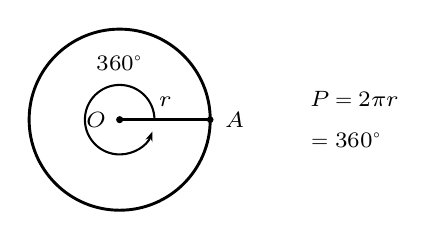
\begin{tikzpicture}[scale=0.92, every node/.style={font=\footnotesize, text=black}]
  \coordinate (O) at (0,0);
  \draw[black, line width=1.05pt] (O) circle (1.25);
  \draw[black, line width=0.95pt] (O) -- (1.25,0) node[midway, above=1pt] {$r$};
  \draw[black, line width=0.75pt, -{Stealth[length=3.5pt]}] (0.48,0) arc (0:340:0.48);
  \fill[black] (O) circle (1.4pt) node[left=1.5pt] {$O$};
  \fill[black] (1.25,0) circle (1.3pt) node[right=2pt] {$A$};
  \node at (0,0.78) {$360^\circ$};
  \node[right=4pt] at (1.55,0.28) {បរិមាត្រ $P = 2\pi r$};
  \node[right=4pt] at (1.55,-0.28) {១ ជុំពេញ $= 360^\circ$};
\end{tikzpicture}}

% ២. E1 Engage: ប្រព័ន្ធបាញ់ទឹកបង្វិលស្រោចដំណាំ ២ កាំ (r1=5m, r2=10m) មុំផ្ចិត 90^\circ
\newcommand{\figEngageCIRCTwo}{%
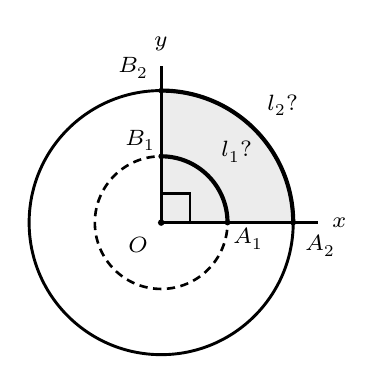
\begin{tikzpicture}[scale=0.78, every node/.style={font=\footnotesize, text=black}]
  \coordinate (O) at (0,0);
  \fill[gray!15] (O) -- (0:2.15) arc (0:90:2.15) -- cycle;
  \draw[black, line width=0.95pt, densely dashed] (O) circle (1.08);
  \draw[black, line width=1.05pt] (O) circle (2.15);
  \draw[black, line width=1.05pt] (O) -- (2.55,0) node[right=1.5pt] {$x$};
  \draw[black, line width=1.05pt] (O) -- (0,2.55) node[above=1.5pt] {$y$};
  \draw[black, line width=1.5pt] (1.08,0) arc (0:90:1.08);
  \draw[black, line width=1.5pt] (2.15,0) arc (0:90:2.15);
  \rightbox[0.22]{0,2.15}{O}{2.15,0}
  \fill[black] (O) circle (1.5pt) node[below left=1.5pt] {$O$};
  \fill[black] (1.08,0) circle (1.3pt) node[below right=1pt, fill=white, inner sep=0.8pt] {$A_1$};
  \fill[black] (0,1.08) circle (1.3pt) node[above left=1pt, fill=white, inner sep=0.8pt] {$B_1$};
  \fill[black] (2.15,0) circle (1.3pt) node[below right=1pt] {$A_2$};
  \fill[black] (0,2.15) circle (1.3pt) node[above left=1pt] {$B_2$};
  \node[above right=1pt] at (45:1.10) {$l_1?$};
  \node[above right=1pt] at (45:2.17) {$l_2?$};
\end{tikzpicture}}

% ៣. E2 Explore: មុំផ្ចិត (មុំលយ vs មុំឆក) និង កាដ្រង់ទាំង ៤ (ទំ.១៩៩)
\newcommand{\figExploreCentralCIRCTwo}{%
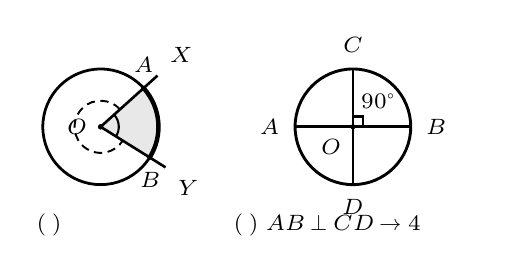
\begin{tikzpicture}[scale=0.72, every node/.style={font=\footnotesize, text=black}]
  % ខាងឆ្វេង៖ មុំផ្ចិតលយ vs មុំផ្ចិតឆក
  \begin{scope}[shift={(0,0)}]
    \coordinate (O) at (1.45,1.42);
    \pgfmathsetmacro{\R}{1.02}
    \fill[gray!18] (O) -- ($(O)+(-32:\R)$) arc (-32:42:\R) -- cycle;
    \draw[black, line width=1.0pt] (O) circle (\R);
    \draw[black, line width=0.95pt] (O) -- ($(O)+(42:1.35)$) node[above right=1pt] {$X$};
    \draw[black, line width=0.95pt] (O) -- ($(O)+(-32:1.35)$) node[below right=1pt] {$Y$};
    \draw[black, line width=1.6pt] ($(O)+(-32:\R)$) arc (-32:42:\R);
    \draw[black, line width=0.75pt] ($(O)+(-32:0.32)$) arc (-32:42:0.32);
    \draw[black, line width=0.7pt, densely dashed] ($(O)+(42:0.46)$) arc (42:328:0.46);
    \fill[black] (O) circle (1.4pt) node[left=1.5pt] {$O$};
    \fill[black] ($(O)+(42:\R)$) circle (1.3pt) node[above=2pt] {$A$};
    \fill[black] ($(O)+(-32:\R)$) circle (1.3pt) node[below=2pt] {$B$};
    \node at (1.50,-0.32) {(ក) មុំផ្ចិតលយ និងឆក};
  \end{scope}
  % ខាងស្ដាំ៖ អង្កត់ផ្ចិតកែងគ្នា AB ⊥ CD -> ៤ កាដ្រង់
  \begin{scope}[shift={(4.45,0)}]
    \coordinate (O) at (1.45,1.42);
    \pgfmathsetmacro{\R}{1.02}
    \draw[black, line width=1.05pt] (O) circle (\R);
    \draw[black, line width=0.95pt] ($(O)+(-\R,0)$) node[left=2pt] {$A$} -- ($(O)+(\R,0)$) node[right=2pt] {$B$};
    \draw[black, line width=0.95pt] ($(O)+(0,-\R)$) node[below=1.5pt] {$D$} -- ($(O)+(0,\R)$) node[above=2pt] {$C$};
    \rightbox[0.18]{$(O)+(0,\R)$}{O}{$(O)+(\R,0)$}
    \fill[black] (O) circle (1.3pt) node[below left=1pt] {$O$};
    \node at ($(O)+(45:0.64)$) {$90^\circ$};
    \node at (1.45,-0.32) {(ខ) $AB\perp CD \to 4$ កាដ្រង់};
  \end{scope}
\end{tikzpicture}}

% ៤. E3 Explain: ធ្នូពីរប៉ុនគ្នាស្កាត់ដោយមុំផ្ចិតពីរប៉ុនគ្នា និងរូបមន្តប្រវែងធ្នូ n^\circ
\newcommand{\figFormulaCIRCTwo}{%
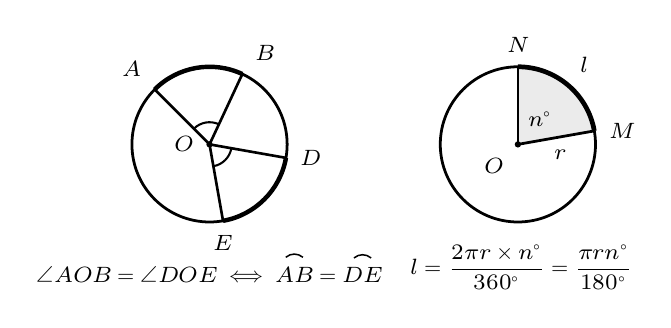
\begin{tikzpicture}[scale=0.88, every node/.style={font=\footnotesize, text=black}]
  % ខាងឆ្វេង៖ ធ្នូប៉ុនគ្នា AB = DE <-> ∠AOB = ∠DOE
  \begin{scope}[shift={(0,0)}]
    \coordinate (O) at (1.40,1.20);
    \pgfmathsetmacro{\R}{1.12}
    \draw[black, line width=1.0pt] (O) circle (\R);
    \draw[black, line width=0.95pt] (O) -- ($(O)+(135:\R)$) node[above left=1pt] {$A$};
    \draw[black, line width=0.95pt] (O) -- ($(O)+(65:\R)$) node[above right=1pt] {$B$};
    \draw[black, line width=0.95pt] (O) -- ($(O)+(-10:\R)$) node[right=1.5pt] {$D$};
    \draw[black, line width=0.95pt] (O) -- ($(O)+(-80:\R)$) node[below=1.5pt] {$E$};
    \draw[black, line width=1.6pt] ($(O)+(65:\R)$) arc (65:135:\R);
    \draw[black, line width=1.6pt] ($(O)+(-80:\R)$) arc (-80:-10:\R);
    \draw[black, line width=0.75pt] ($(O)+(65:0.32)$) arc (65:135:0.32);
    \draw[black, line width=0.75pt] ($(O)+(-80:0.32)$) arc (-80:-10:0.32);
    \fill[black] (O) circle (1.3pt) node[left=2pt] {$O$};
    \node at (1.40,-0.58) {$\ang{AOB}=\ang{DOE} \iff \arc{AB}=\arc{DE}$};
  \end{scope}
  % ខាងស្ដាំ៖ រូបមន្តប្រវែងធ្នូ l
  \begin{scope}[shift={(4.45,0)}]
    \coordinate (O) at (1.40,1.20);
    \pgfmathsetmacro{\R}{1.12}
    \fill[gray!16] (O) -- ($(O)+(10:\R)$) arc (10:90:\R) -- cycle;
    \draw[black, line width=1.0pt] (O) circle (\R);
    \draw[black, line width=1.0pt] (O) -- ($(O)+(10:\R)$) node[right=1.5pt] {$M$};
    \draw[black, line width=1.0pt] (O) -- ($(O)+(90:\R)$) node[above=1.5pt] {$N$};
    \draw[black, line width=1.7pt] ($(O)+(10:\R)$) arc (10:90:\R);
    \node at ($(O)+(48:0.48)$) {$n^\circ$};
    \node[below=1pt] at ($(O)+(10:0.62)$) {$r$};
    \node[above right=1pt] at ($(O)+(50:\R)$) {$l$};
    \fill[black] (O) circle (1.3pt) node[below left=1.5pt] {$O$};
    \node at (1.45,-0.58) {$l = \dfrac{2\pi r \times n^\circ}{360^\circ} = \dfrac{\pi r n^\circ}{180^\circ}$};
  \end{scope}
\end{tikzpicture}}

% ៥. E4 Elaborate: លំហាត់គំរូទី១ (r=10 dm, 36^\circ) និង ទី២ (r=15 cm, 80^\circ)
\newcommand{\figModelCIRCTwo}{%
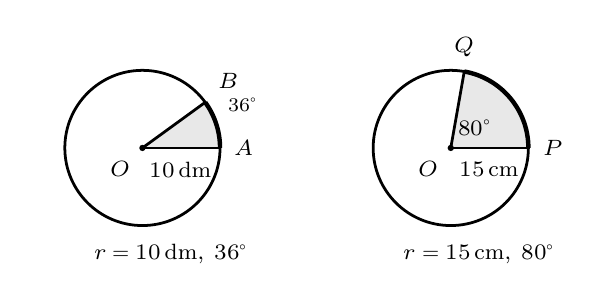
\begin{tikzpicture}[scale=0.88, every node/.style={font=\footnotesize, text=black}]
  % គំរូទី១៖ r=10 dm, 36^\circ
  \begin{scope}[shift={(0,0)}]
    \coordinate (O) at (1.35,1.15);
    \pgfmathsetmacro{\R}{1.12}
    \fill[gray!18] (O) -- ($(O)+(0:\R)$) arc (0:36:\R) -- cycle;
    \draw[black, line width=1.0pt] (O) circle (\R);
    \draw[black, line width=1.0pt] (O) -- ($(O)+(0:\R)$) node[right=1.5pt] {$A$};
    \draw[black, line width=1.0pt] (O) -- ($(O)+(36:\R)$) node[above right=1pt] {$B$};
    \draw[black, line width=1.6pt] ($(O)+(0:\R)$) arc (0:36:\R);
    \fill[black] (O) circle (1.3pt) node[below left=1pt] {$O$};
    \node[below=1.5pt] at ($(O)+(0:0.55)$) {$10\unit{dm}$};
    \node[above right=1pt, font=\scriptsize] at ($(O)+(18:1.12)$) {$36^\circ$};
    \node at (1.35,-0.38) {គំរូទី១៖ $r=10\unit{dm},\; 36^\circ$};
  \end{scope}
  % គំរូទី២៖ r=15 cm, 80^\circ
  \begin{scope}[shift={(4.45,0)}]
    \coordinate (O) at (1.35,1.15);
    \pgfmathsetmacro{\R}{1.12}
    \fill[gray!18] (O) -- ($(O)+(0:\R)$) arc (0:80:\R) -- cycle;
    \draw[black, line width=1.0pt] (O) circle (\R);
    \draw[black, line width=1.0pt] (O) -- ($(O)+(0:\R)$) node[right=1.5pt] {$P$};
    \draw[black, line width=1.0pt] (O) -- ($(O)+(80:\R)$) node[above=1.5pt] {$Q$};
    \draw[black, line width=1.6pt] ($(O)+(0:\R)$) arc (0:80:\R);
    \fill[black] (O) circle (1.3pt) node[below left=1pt] {$O$};
    \node[below=1.5pt] at ($(O)+(0:0.55)$) {$15\unit{cm}$};
    \node at ($(O)+(40:0.45)$) {$80^\circ$};
    \node at (1.35,-0.38) {គំរូទី២៖ $r=15\unit{cm},\; 80^\circ$};
  \end{scope}
\end{tikzpicture}}

% ៦. E5 Practice (ទំ.២០០)៖ ធ្នូ AB < ធ្នូ CD
\newcommand{\figPracticeCIRCTwo}{%
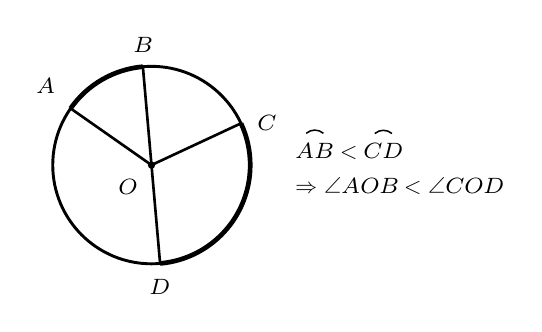
\begin{tikzpicture}[scale=0.95, every node/.style={font=\footnotesize, text=black}]
  \coordinate (O) at (0,0);
  \pgfmathsetmacro{\R}{1.32}
  \draw[black, line width=1.05pt] (O) circle (\R);
  \draw[black, line width=0.95pt] (O) -- (145:\R) node[above left=1.5pt] {$A$};
  \draw[black, line width=0.95pt] (O) -- (95:\R) node[above=1.5pt] {$B$};
  \draw[black, line width=0.95pt] (O) -- (25:\R) node[right=2pt] {$C$};
  \draw[black, line width=0.95pt] (O) -- (-85:\R) node[below=2pt] {$D$};
  \draw[black, line width=1.7pt] (95:\R) arc (95:145:\R);
  \draw[black, line width=1.7pt] (-85:\R) arc (-85:25:\R);
  \fill[black] (O) circle (1.4pt) node[below left=1.5pt] {$O$};
  \node[right=4pt] at (1.65,0.28) {$\arc{AB} < \arc{CD}$};
  \node[right=4pt] at (1.65,-0.28) {$\Rightarrow \ang{AOB} < \ang{COD}$};
\end{tikzpicture}}

% ៧. កិច្ចការផ្ទះ៖ លំហាត់ទី១ (ទំ.២០៤) ∠OAB = 25^\circ -> ∠AOB = 130^\circ
\newcommand{\figHWCIRCTwo}{%
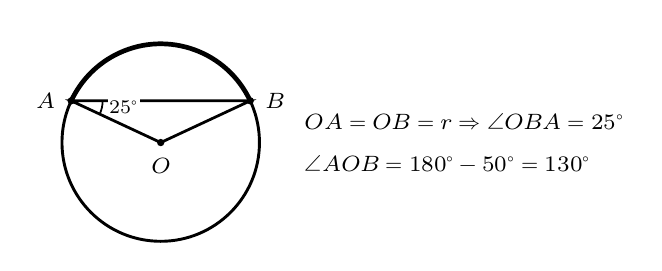
\begin{tikzpicture}[scale=0.95, every node/.style={font=\footnotesize, text=black}]
  \coordinate (O) at (0,0);
  \pgfmathsetmacro{\R}{1.32}
  \coordinate (A) at (155:\R);
  \coordinate (B) at (25:\R);
  \draw[black, line width=1.05pt] (O) circle (\R);
  \draw[black, line width=1.0pt] (O) -- (A) -- (B) -- cycle;
  \draw[black, line width=1.7pt] (B) arc (25:155:\R);
  \fill[black] (O) circle (1.4pt) node[below=2pt] {$O$};
  \fill[black] (A) circle (1.4pt) node[left=2pt] {$A$};
  \fill[black] (B) circle (1.4pt) node[right=2pt] {$B$};
  \draw[black, line width=0.65pt] ($(A)+(0:0.42)$) arc (0:-25:0.42);
  \node[right=1.5pt, font=\scriptsize, fill=white, inner sep=0.6pt] at ($(A)+(-12:0.44)$) {$25^\circ$};
  \node[right=4pt] at (1.65,0.28) {$OA=OB=r \Rightarrow \ang{OBA}=25^\circ$};
  \node[right=4pt] at (1.65,-0.28) {$\ang{AOB}=180^\circ-50^\circ=130^\circ$};
\end{tikzpicture}}

% ============================================================================
% ចាប់ផ្ដើមឯកសារ (Document Body)
% ============================================================================
\begin{document}
\fontsize{10pt}{15.2pt}\selectfont

% -------------------- ក្បាលកិច្ចតែងការ (Header) --------------------
\begin{center}
  {\muol\fontsize{11pt}{16pt}\selectfont ព្រះរាជាណាចក្រកម្ពុជា}\\[2pt]
  {\muol\fontsize{10pt}{15pt}\selectfont ជាតិ សាសនា ព្រះមហាក្សត្រ}\\[1pt]
  \khmflourish
\end{center}

\vspace{-28pt}
{\muol\fontsize{9.5pt}{12.5pt}\selectfont
មន្ទីរអប់រំ យុវជន និងកីឡា ខេត្តកំពង់ធំ\\
ការិយាល័យអប់រំ យុវជន និងកីឡា ស្រុកកំពង់ស្វាយ\\
អនុវិទ្យាល័យព្រះក្រសាំង}

\vspace{1pt}
\begin{center}
  {\muol\fontsize{10pt}{14pt}\selectfont កិច្ចតែងការបង្រៀន}
\end{center}
\vspace{0pt}

% -------------------- ព័ត៌មានទូទៅ (Metadata) --------------------
{\renewcommand{\arraystretch}{0.95}
\hspace*{4.05cm}%
\begin{tabular}{@{}l l l@{}}
  - \hspace{0.35cm} មុខវិជ្ជា & : & គណិតវិទ្យា ថ្នាក់ទី៨ \\
  - \hspace{0.35cm} ចំណងជើងមេរៀន & : & មេរៀនទី១៥ រង្វង់ \\
  - \hspace{0.35cm} ចំណងជើងរង & : & ២.១ មុំផ្ចិត និងរង្វាស់ប្រវែងធ្នូនៃរង្វង់ (ទំ.១៩៩--២០០) \\
  - \hspace{0.35cm} រយៈពេល & : & ១ ម៉ោងសិក្សា (៥០ នាទី) \\
  - \hspace{0.35cm} បង្រៀនដោយ & : & ហុក ប៊ុនថែន \\
  - \hspace{0.35cm} កាលបរិច្ឆេទ & : & ថ្ងៃអង្គារ ទី១៥ ខែធ្នូ ឆ្នាំ២០២៦ \\
\end{tabular}

\vspace{1pt}

% -------------------- I. វត្ថុបំណង --------------------
\textbf{I.} {\muol វត្ថុបំណង}\\[1pt]
\hspace*{0.55cm}%
\begin{tabular}{@{}l l L{14.2cm}@{}}
  \wcirc \hspace{0.25cm} វិជ្ជាសម្បទា & : & សិស្សប្រាប់និយមន័យមុំផ្ចិត (មុំលយ និងមុំឆក) ធ្នូស្កាត់ដោយមុំផ្ចិត កាដ្រង់នៃរង្វង់ លក្ខណៈធ្នូពីរប៉ុនគ្នា និងរូបមន្តប្រវែងធ្នូ $l = \frac{2\pi r \times n^\circ}{360^\circ}$ ដោយបែងចែកដាច់ពីរង្វាស់ដឺក្រេនៃធ្នូបានត្រឹមត្រូវ ។ \\
  \wcirc \hspace{0.25cm} បំណិនសម្បទា & : & សិស្សវាស់មុំផ្ចិតដោយរ៉ាប់ព័រទ័រលើសន្លឹកកិច្ចការ បង្កើតរូបមន្តប្រវែងធ្នូតាមតារាងសមាមាត្រទ្វេ និងគណនាប្រវែងធ្នូនៃរង្វង់ក្នុងលំហាត់គំរូ និងជីវភាពជាក់ស្ដែងបានត្រឹមត្រូវ ។ \\
  \wcirc \hspace{0.25cm} ចរិយាសម្បទា & : & សិស្សមានស្មារតីសហការពិភាក្សាក្នុងក្រុម ផ្ទៀងផ្ទាត់ឯកតារង្វាស់ប្រវែងយ៉ាងហ្មត់ចត់ និងយល់ឃើញសារៈសំខាន់នៃរូបមន្តធ្នូរង្វង់ក្នុងបច្ចេកទេសកសិកម្មនិងសំណង់ ។ \\
\end{tabular}

\vspace{1pt}

% -------------------- II. សម្ភារៈឧបទេស --------------------
\textbf{II.} {\muol សម្ភារៈឧបទេស}\\[1pt]
\hspace*{0.55cm}$\bullet$ \hspace{0.35cm} សៀវភៅសិក្សាគោលថ្នាក់ទី៨ (ទំ.១៩៩--២០០, ២០៤) ក្ដារខៀន ដីស បន្ទាត់ក្រិត រ៉ាប់ព័រទ័រ និងដែកឈានក្ដារខៀន ព្រមទាំង\textbf{សន្លឹកកិច្ចការសិស្ស ស-ខ្មៅ (\en{Worksheet\_CIRC2} ទំព័រ ១--២)} (បង្រៀនដោយគ្មានស្លាយ \en{LCD})

\vspace{1pt}

% -------------------- III. វិធីសាស្រ្តបង្រៀន --------------------
\textbf{III.} {\muol វិធីសាស្រ្តបង្រៀន}\\[1pt]
\hspace*{0.45cm}%
\begin{tabular}{@{}l l L{14.85cm}@{}}
  $\bullet$ \hspace{0.25cm} គោលវិធី & : & សិស្សមជ្ឈមណ្ឌល (ផ្អែកលើសន្លឹកកិច្ចការរុករក ស-ខ្មៅ ជាគោល គ្មានស្លាយ \en{LCD}) \\
  $\bullet$ \hspace{0.25cm} យុទ្ធវិធីបង្រៀន & : & គំរូ 5Es រួមផ្សំសន្លឹកកិច្ចការរុករកជាក្រុម (\en{POGIL}) និងតារាងសមាមាត្រទ្វេ (\en{Double-Scale Proportional Ratio Table}) បំបែកការភាន់ច្រឡំរវាងរង្វាស់ដឺក្រេ និងប្រវែងធ្នូ \\
\end{tabular}
}

\vspace{1pt}

% -------------------- IV. ដំណើរការបង្រៀន --------------------
\textbf{IV.} {\muol ដំណើរការបង្រៀន}

\vspace{1pt}

\renewcommand{\arraystretch}{1.15}
\begin{longtable}{|L{5.50cm}|L{7.90cm}|L{4.80cm}|}
\hline
\rowcolor{headgray}
\multicolumn{1}{|c|}{\muol សកម្មភាពគ្រូ} &
\multicolumn{1}{c|}{\muol ខ្លឹមសារមេរៀន} &
\multicolumn{1}{c|}{\muol សកម្មភាពសិស្ស} \\
\hline
\endfirsthead

\hline
\endhead

\hline
\endfoot

\hline
\endlastfoot

% ==================== ជំហានទី១ (2min) ====================
\stepheader{ជំហានទី១ \enbf{(}រដ្ឋបាលថ្នាក់\enbf{)}}
$\bullet$ ពិនិត្យអវត្តមាន សណ្ដាប់ធ្នាប់ អនាម័យ និងការត្រៀមរ៉ាប់ព័រទ័រ បន្ទាត់ក្រិត ដែកឈាន
&
$\bullet$ រដ្ឋបាលថ្នាក់ និងការត្រៀមរ៉ាប់ព័រទ័រវាស់មុំលើសន្លឹកកិច្ចការ
&
$\circ$ ប្រធានថ្នាក់រាយការណ៍អវត្តមាន និងត្រៀមរ៉ាប់ព័រទ័រ បន្ទាត់ \\[3pt]

$\bullet$ ចែក \textbf{សន្លឹកកិច្ចការ ១៥.២} (ទំព័រ ១--២) ជូនសិស្សតាមក្រុមតូច ៣ នាក់ ផ្កាប់លើតុ
&
$\bullet$ សន្លឹកកិច្ចការរុករកតាមបែប \en{POGIL} និងតារាងសមាមាត្រទ្វេ
&
$\circ$ ទទួលសន្លឹកកិច្ចការផ្កាប់ទុកលើតុតាមក្រុម \\
\hline

% ==================== ជំហានទី២ (9min: <=3 + 3 + E1 3) ====================
\stepheader{ជំហានទី២ \enbf{(}ពិនិត្យចំណេះដឹងមុន \enbf{+} ទំនាក់ទំនងមេរៀនថ្មី\enbf{)}}
\ditem \textbf{ពិនិត្យកិច្ចការផ្ទះ ($\le 3\unit{min}$)} \timenote{ផ្ទៀងគន្លឹះខ្លីលើក្ដារ} \par
$\bullet$ ហៅសិស្ស ២ នាក់ឆ្លើយផ្ទាល់មាត់ពីតម្រុយលំហាត់ទី៦ និងទី៧ (ទំ.២០៤) ពីម៉ោងមុន
&
{\centering\redsub{កំណែសង្ខេបលំហាត់ទី៦ និងទី៧ (ទំ.២០៤)}\par} \par
$\bullet$ \textbf{ទី៦៖} $JB=JI=JK=JC=\frac{BC}{2} \Rightarrow B,I,K,C \in C(J,\frac{BC}{2})$ ។ \par
$\bullet$ \textbf{ទី៧៖} $MNRS$ ជាចតុកោណកែង មានអង្កត់ទ្រូងស្មើគ្នានិងកាត់ចំកណ្ដាលគ្នាត្រង់ $O \Rightarrow OM=ON=OR=OS$ ។
&
$\circ$ ផ្ទៀងផ្ទាត់ចម្លើយក្នុងសៀវភៅកិច្ចការផ្ទះយ៉ាងរហ័ស \\[3pt]

\ditem \textbf{រំលឹកមេរៀនទាក់ទង (3min)} \timenote{សរុបកុំឱ្យលើស 3min} \par
$\bullet$ គូសរង្វង់ $C(O,r)$ លើក្ដារខៀន រួចសួររូបមន្តបរិមាត្ររង្វង់
&
{\centering\redsub{រំលឹកបរិមាត្ររង្វង់ និងមុំពេញជុំវិញផ្ចិត}\par} \par
$\bullet$ បរិមាត្ររង្វង់កាំ $r$ គឺ \graybox{$P = 2\pi r = \pi d$} ($\pi \approx 3.14$) ។
&
$\circ$ ឆ្លើយផ្ទាល់មាត់៖ «បរិមាត្ររង្វង់គឺ $P=2\pi r$!» \\[3pt]

– \textbf{សំណួរ៖} តើរង្វាស់មុំពេញជុំវិញផ្ចិត $O$ មួយជុំ កន្លះជុំ និងមួយភាគបួនជុំស្មើប៉ុន្មានដឺក្រេ?
&
$\bullet$ មុំពេញមួយជុំ $= 360^\circ$, កន្លះជុំ $= 180^\circ$, មួយភាគបួនជុំ $= 90^\circ$ ។
&
$\circ$ ឆ្លើយ៖ «$360^\circ, 180^\circ$ និង $90^\circ$!» \\[3pt]

&
\cfig{\figPrereqCIRCTwo}
& \\[3pt]

\fiveE{E1 - Engage (3min)} \timenote{(បំផុសចម្ងល់ — កុំទាន់ផ្ដល់ចម្លើយ)} \par
\ditem \textbf{បញ្ហាជីវភាពពិត (ក្បាលបាញ់ទឹកស្រោចដំណាំវិលជុំ)៖} \par
គូសរង្វង់រួមផ្ចិតពីរ ($r_1=5\unit{m}$ និង $r_2=10\unit{m}$) ដែលក្បាលបាញ់ទឹកវិលបានមុំកែង $90^\circ$
&
{\centering\redsub{បេសកកម្ម៖ មុំបង្វិលដូចគ្នា តើប្រវែងធ្នូស្មើគ្នាឬទេ?}\par}
&
$\circ$ សង្កេតរូបក្បាលបាញ់ទឹកលើក្ដារខៀន និងផ្នែកក្បាលសន្លឹកកិច្ចការ \\[3pt]

&
\cfig{\figEngageCIRCTwo}
& \\[3pt]

– \textbf{សំណួរបំផុស៖} បើក្បាលបាញ់ទឹកវិលបានមុំ $90^\circ$ ដូចគ្នា តើធ្នូទឹក $\arc{A_1B_1}$ និង $\arc{A_2B_2}$ មាន\textbf{រង្វាស់ដឺក្រេ}ស្មើគ្នាទេ? ចុះ\textbf{ប្រវែងគិតជាម៉ែត្រ}ស្មើគ្នាដែរឬទេ?
&
\textbf{ចម្ងល់គោល៖} \par
$\bullet$ រង្វាស់ដឺក្រេនៃធ្នូ ($\text{m}\arc{AB} = n^\circ$) ខុសពីប្រវែងធ្នូ ($l$) យ៉ាងដូចម្ដេច? \par
$\bullet$ បើស្គាល់កាំ $r$ និងមុំផ្ចិត $n^\circ$ តើគណនាប្រវែងធ្នូ $l$ តាមរូបមន្តអ្វី?
&
$\circ$ ពិភាក្សាទស្សន៍ទាយក្នុងក្រុម និងកត់ចម្លើយទាយលើសន្លឹកកិច្ចការ \\
\hline

% ==================== ជំហានទី៣ (17min: E2 11m + E3 6m) ====================
\stepheader{ជំហានទី៣ \enbf{(}ខ្លឹមសារមេរៀនថ្មី\enbf{)}}
\fiveE{E2 - Explore (11min)} \par
$\bullet$ សរសេរចំណងជើងមេរៀនរងលើក្ដារខៀន និងឱ្យសិស្សបើក \textbf{សន្លឹកកិច្ចការ ទំព័រ ១ (ផ្នែក ក)}
&
២. មុំផ្ចិត និងធ្នូ \par
២.១ មុំផ្ចិត កាដ្រង់ និងរង្វាស់ប្រវែងធ្នូនៃរង្វង់ (ទំ.១៩៩--២០០)
&
$\circ$ កត់ចំណងជើង និងបើកសន្លឹកកិច្ចការទំព័រ ១ \\[3pt]

\ditem \textbf{សកម្មភាព POGIL ទី១ (5min)៖ វាស់មុំផ្ចិត និងស្គាល់កាដ្រង់ (ទំ.១៩៩)} \par
$\bullet$ ឱ្យសិស្សប្រើរ៉ាប់ព័រទ័រវាស់មុំផ្ចិតលយ $\ang{A_2OB_2}$ និងមុំផ្ចិតឆកលើសន្លឹកកិច្ចការ
&
$\bullet$ \textbf{ឧទាហរណ៍ទី១៖} មុំដែលមានកំពូលត្រង់ផ្ចិត $O$ នៃរង្វង់ ហៅថា\textbf{មុំផ្ចិត} (មានមុំលយ និងមុំឆក) ។ ចំណុច $A, B$ ហៅថា\textbf{ចុងធ្នូ} ហើយ $\arc{AB}$ ជា\textbf{ធ្នូស្កាត់ដោយមុំផ្ចិត} ។
&
$\circ$ ប្រើរ៉ាប់ព័រទ័រវាស់មុំផ្ចិតលយ និងគណនាមុំផ្ចិតឆកលើសន្លឹកកិច្ចការ \\[3pt]

$\bullet$ ឱ្យសិស្សពិនិត្យអង្កត់ផ្ចិតកែងគ្នា $AB\perp CD$ និងរាប់ចំនួនកាដ្រង់នៃរង្វង់
&
$\bullet$ \textbf{ឧទាហរណ៍ទី៣៖} បើអង្កត់ផ្ចិត $AB \perp CD$ គេបានមុំកែង $90^\circ$ បួន ចែករង្វង់ជា ៤ ធ្នូប៉ុនគ្នា ដែលធ្នូនីមួយៗហៅថា \graybox{កាដ្រង់} ។
&
$\circ$ កំណត់ចុងធ្នូ និងកាដ្រង់ទាំង ៤ លើរូបសន្លឹកកិច្ចការ \\[3pt]

&
\cfig{\figExploreCentralCIRCTwo}
& \\[3pt]

\ditem \textbf{សកម្មភាព POGIL ទី២ (6min)៖ តារាងសមាមាត្រទ្វេបង្កើតរូបមន្តប្រវែងធ្នូ} \par
$\bullet$ ដឹកនាំសិស្សបំពេញ\textbf{តារាងសមាមាត្រទ្វេ}លើសន្លឹកកិច្ចការ៖ ពី $360^\circ \to 180^\circ \to 90^\circ \to 1^\circ$
&
{\centering\textbf{តារាងសមាមាត្រទ្វេរកប្រវែងធ្នូ $l$}\par} \par
$\bullet$ ធ្នូពេញរង្វង់ ($360^\circ$) មានប្រវែងស្មើបរិមាត្រ $P = 2\pi r$ ។ \par
$\bullet$ ធ្នូ $1^\circ$ មានប្រវែង $= \dfrac{2\pi r}{360^\circ}$ ។
&
$\circ$ គណនាប្រវែងធ្នូ $180^\circ, 90^\circ$ និង $1^\circ$ តាមសមាមាត្រក្នុងតារាង \\[3pt]

$\bullet$ ឱ្យសិស្សទាញរូបមន្តទូទៅសម្រាប់មុំផ្ចិត $n^\circ$ និងសម្រួលនឹង $2$
&
$\bullet$ ធ្នូ $n^\circ$ មានប្រវែង \graybox{$l = \dfrac{2\pi r \times n^\circ}{360^\circ} = \dfrac{\pi r n^\circ}{180^\circ}$} ។
&
$\circ$ ទាញរូបមន្ត $l$ និងឃើញថាបើ $r$ ធំជាង ប្រវែងធ្នូ $l$ វែងជាង! \\[3pt]

% --- E3 Explain (6min) ---
\fiveE{E3 - Explain (6min)} \par
\ditem \textbf{សំយោគលក្ខណៈទូទៅ និងរូបមន្តប្រវែងធ្នូ (ទំ.១៩៩)} \par
$\bullet$ ឱ្យតំណាងក្រុមឡើងបង្ហាញតារាងសមាមាត្រ រួចគ្រូសង្ខេបលក្ខណៈទូទៅ (ឧទាហរណ៍ទី២) លើក្ដារខៀន
&
\textbf{ជាទូទៅ (ទំ.១៩៩)៖} ក្នុងរង្វង់មួយ ឬរង្វង់ពីរប៉ុនគ្នា \textbf{ធ្នូពីរប៉ុនគ្នាស្កាត់ដោយមុំផ្ចិតពីរប៉ុនគ្នា} ហើយច្រាសមកវិញ \textbf{បើមុំផ្ចិតពីរប៉ុនគ្នា នោះធ្នូស្កាត់ទាំងពីរប៉ុនគ្នា} ($\ang{AOB}=\ang{DOE} \iff \arc{AB}=\arc{DE}$) ។ \par
\textbf{សម្គាល់៖} ធ្នូមួយដឺក្រេ ($1^\circ$) ជាធ្នូស្កាត់ដោយមុំផ្ចិត $1^\circ$ ។
&
$\circ$ បំពេញប្រអប់ «ជាទូទៅ» និងរូបមន្តក្នុងផ្នែក ខ នៃសន្លឹកកិច្ចការទំព័រ ១ \\[3pt]

&
\cfig{\figFormulaCIRCTwo}
& \\[3pt]

$\bullet$ សង្ខេប\textbf{ធនាគារហេតុផល \cnum{1}--\cnum{5}} និងបញ្ជាក់ភាពខុសគ្នារវាង $\text{m}\arc{AB}=n^\circ$ (គិតជាដឺក្រេ) និង $l$ (គិតជា $\text{cm, dm, m}$)
&
\textbf{ធនាគារហេតុផល៖} \cnum{1} និយមន័យមុំផ្ចិត ($\text{m}\arc{AB}=\ang{AOB}$) \textbar{} \cnum{2} អង្កត់ផ្ចិតកែងគ្នា ($4$ កាដ្រង់ $90^\circ$) \textbar{} \cnum{3} មុំផ្ចិតប៉ុនគ្នា $\iff$ ធ្នូប៉ុនគ្នា \textbar{} \cnum{4} បរិមាត្រ $P=2\pi r$ \textbar{} \cnum{5} ប្រវែងធ្នូ $l=\frac{2\pi r \cdot n^\circ}{360^\circ}$ ។
&
$\circ$ កត់ត្រាចំណុចខុសគ្នារវាងរង្វាស់ដឺក្រេ ($^\circ$) និងប្រវែងធ្នូ ($l$) \\
\hline

% ==================== ជំហានទី៤ (20min: E4 10m + E5 10m) ====================
\stepheader{ជំហានទី៤ \enbf{(}ពង្រីកចំណេះដឹង\enbf{)}}
\fiveE{E4 - Elaborate (10min)} \par
\ditem \textbf{លំហាត់គំរូទី១ និង ទី២ (ទំ.១៩៩--២០០) — សន្លឹកកិច្ចការទំព័រ ២ (ផ្នែក គ)} \par
$\bullet$ ដឹកនាំសិស្សដោះស្រាយ \textbf{លំហាត់គំរូទី១} ($r=10\unit{dm}, n^\circ=36^\circ$) ដោយបញ្ជាក់ច្បាស់ពីតម្លៃប្រហែលនៃ $\pi$
&
{\muol លំហាត់គំរូទី១} \textbf{(ទំ.១៩៩--២០០)៖} រង្វង់មានកាំ $r=10\unit{dm}$ ។ គណនាប្រវែងធ្នូស្កាត់ដោយមុំផ្ចិត $36^\circ$ ។ \par
$\bullet$ បរិមាត្ររង្វង់៖ $P = 2\pi r = 20\pi\unit{dm}$ ។ \par
$\bullet$ បើយក $\pi \approx 3.14 \Rightarrow P \approx 62.8\unit{dm} \Rightarrow l = \frac{62.8 \times 36^\circ}{360^\circ} = \graybox{$6.28\unit{dm}$}$ (\textit{បើយក $\pi\approx 3.1416$ តាមសៀវភៅគោល បាន $l \approx 6.2832\unit{dm}$}) ។
&
$\circ$ គូស \textbf{[tracing]} លើមុំផ្ចិត $36^\circ$ និងគណនាតាមតារាងសមាមាត្រលើសន្លឹកកិច្ចការ \\[3pt]

&
\cfig{\figModelCIRCTwo}
& \\[3pt]

$\bullet$ ឱ្យសិស្សធ្វើ \textbf{លំហាត់គំរូទី២} ($r=15\unit{cm}, n^\circ=80^\circ, \pi=3.14$) និងឱ្យសិស្សចាប់កំហុសឯកតាក្នុងសៀវភៅគោលទំព័រ ២០០ (\en{dm} $\to$ \en{cm})
&
{\muol លំហាត់គំរូទី២} \textbf{(ទំ.២០០)៖} $r=15\unit{cm}, n^\circ=80^\circ (\pi=3.14)$ ៖ \par
$\bullet$ បរិមាត្រ៖ $P = 2 \times 3.14 \times 15 = 94.2\unit{cm}$ (\textit{កែតម្រូវកំហុសបោះពុម្ពទំ.២០០ ពី $94.2\unit{dm}$ មក $94.2\unit{cm}$}) ។
&
$\circ$ គណនាបរិមាត្រ $P=94.2\unit{cm}$ និងផ្ទៀងឯកតា $\text{cm}$ \\[3pt]

– \textbf{សំណួរ EIA 30s៖} ហេតុអ្វីដឺក្រេ $^\circ$ រលុបបាត់ ហើយនៅសល់តែឯកតាប្រវែង $\text{cm}$?
&
$\bullet$ ប្រវែងធ្នូ៖ $l = \dfrac{94.2\unit{cm} \times 80^\circ}{360^\circ} = \dfrac{62.8}{3} \approx \graybox{$20.93\unit{cm}$}$ ។ \par
\timenote{EIA 30s៖ ព្រោះផលធៀប $\frac{80^\circ}{360^\circ}=\frac{2}{9}$ គ្មានឯកតា (ជាប្រភាគនៃរង្វង់)!}
&
$\circ$ គណនាប្រវែងធ្នូ $l \approx 20.93\unit{cm}$ និងឆ្លើយសំណួរ EIA 30s \\[3pt]

\fiveE{E5 - Evaluate (10min)} \par
\ditem {\muol លំហាត់ប្រតិបត្តិ} \textbf{(6.5min — សន្លឹកកិច្ចការទំព័រ ២ ផ្នែក ឃ)} \par
$\bullet$ ឱ្យសិស្សប្រើរ៉ាប់ព័រទ័រវាស់មុំផ្ចិត $\ang{AOB}$ និង $\ang{COD}$ លើរង្វង់ដែលមាន $\arc{AB} < \arc{CD}$ រួចគណនាប្រវែងធ្នូទាំងពីរ
&
{\muol លំហាត់ប្រតិបត្តិ} \textbf{(ទំ.២០០)៖} រង្វង់ផ្ចិត $O$ មានធ្នូតូចពីរមិនប៉ុនគ្នា $\arc{AB} < \arc{CD}$ ៖ \par
$\bullet$ វាស់លើរូបខ្នាតពិត៖ $\ang{AOB} = 50^\circ$ និង $\ang{COD} = 110^\circ \Rightarrow \ang{AOB} < \ang{COD}$ ។ \par
$\bullet$ \textbf{សន្និដ្ឋាន៖} ក្នុងរង្វង់តែមួយ ធ្នូតូចណាខ្លីជាង ស្កាត់ដោយមុំផ្ចិតតូចជាង ($\arc{AB} < \arc{CD} \iff \ang{AOB} < \ang{COD}$) ។
&
$\circ$ ប្រើរ៉ាប់ព័រទ័រវាស់ $\ang{AOB}, \ang{COD}$ គណនាប្រវែងធ្នូ និងសរសេរសេចក្ដីសន្និដ្ឋាន \\[3pt]

&
\cfig{\figPracticeCIRCTwo}
& \\[3pt]

\ditem \textbf{បិទបញ្ហា E1 និងសំណួរវិនិច្ឆ័យរហ័ស A--D (3.5min — ផ្នែក ង)} \par
$\bullet$ ឱ្យសិស្សឆ្លើយបិទបញ្ហាក្បាលបាញ់ទឹក E1 ($r_1=5\unit{m}, r_2=10\unit{m}, 90^\circ$) និងគូសធីកប្រអប់ A--D
&
$\bullet$ \textbf{បិទ E1៖} ធ្នូទាំងពីរមានរង្វាស់ដឺក្រេ $90^\circ$ ស្មើគ្នា តែប្រវែងខុសគ្នាគឺ $l_1 \approx 7.85\unit{m}$ និង $l_2 \approx 15.70\unit{m}$ ($l_2 = 2l_1$) ។ \par
$\bullet$ \textbf{ចម្លើយរហ័ស A--D៖} A (\ding{51} កាដ្រង់ $=90^\circ$) \textbar{} B (\ding{55} ប្រវែងធ្នូអាស្រ័យលើកាំ $r$ ផងដែរ) \textbar{} C (\ding{51} $60^\circ = \frac{1}{6}$ នៃបរិមាត្រ) \textbar{} D (\ding{51} $\arc{AB}=\arc{DE}\iff \ang{AOB}=\ang{DOE}$) ។
&
$\circ$ បំពេញប្រអប់ A--D និងផ្ទៀងចម្លើយជាមួយគ្រូ \\
\hline

% ==================== ជំហានទី៥ (<=2min) ====================
\stepheader{ជំហានទី៥ \enbf{(}កិច្ចការផ្ទះ \enbf{+} បណ្ដាំផ្ញើ\enbf{)}}
\timenote{ចំណាយពេលឱ្យតិចបំផុតកុំឱ្យលើស 2min} \par
$\bullet$ ដាក់កិច្ចការផ្ទះ \textbf{លំហាត់ទី១ (ទំ.២០៤)} នៅផ្នែកចុងក្រោយនៃសន្លឹកកិច្ចការទំព័រ ២
&
{\centering{\muol កិច្ចការផ្ទះ} \textbf{(សៀវភៅគោល ទំ.២០៤ ៖ លំហាត់ទី១ + អនុវត្តប្រវែងធ្នូ)}\par} \par
$\bullet$ \textbf{១. លំហាត់ទី១ (ទំ.២០៤)៖} ក្នុងរង្វង់ $C(O,r)$ ត្រីកោណ $OAB$ មានមុំ $\ang{OAB}=25^\circ$ ។ គណនារង្វាស់ដឺក្រេនៃធ្នូតូច $\arc{AB}$ (\textit{តម្រុយ៖ $\tri{OAB}$ សមបាទកំពូល $O \Rightarrow \ang{AOB}=130^\circ$}) ។
&
$\circ$ កត់ត្រាតម្រុយលំហាត់ទី១ លើសន្លឹកកិច្ចការ \\[3pt]

&
\cfig{\figHWCIRCTwo}
& \\[3pt]

$\bullet$ ណែនាំបន្តលំហាត់អនុវត្តគណនាប្រវែងធ្នូនៅផ្ទះ និងផ្ដាំផ្ញើសិស្សអានមុនចំណុច \textbf{២.២ ធ្នូ និងអង្កត់ធ្នូ (ទំ.២០០--២០១)}
&
$\bullet$ \textbf{២. អនុវត្ត៖} បើរង្វង់ខាងលើមានកាំ $r = 18\unit{cm}$ ចូរគណនាប្រវែងធ្នូតូច $\arc{AB}$ គិតជា $\text{cm}$ ($\pi \approx 3.14$) ។ \par
$\bullet$ អានជាមុន៖ \textbf{ធ្នូ និងអង្កត់ធ្នូ} (ទំ.២០០--២០១)
&
$\circ$ កត់ត្រាលំហាត់អនុវត្ត ទទួលបណ្ដាំផ្ញើ និងជម្រាបលាគ្រូ \\
\end{longtable}

% -------------------- កាលបរិច្ឆេទ និងហត្ថលេខា (Date & Signature) --------------------
\vspace{14pt}
\hfill
\begin{minipage}{9.8cm}
  {\centering
    ថ្ងៃអង្គារ ៦កើត ខែមិគសិរ ឆ្នាំមមី អដ្ឋស័ក ពុទ្ធសករាជ ២៥៧០\\[3pt]
    កំពង់ស្វាយ, ថ្ងៃទី១៥ ខែធ្នូ ឆ្នាំ២០២៦\\[4pt]
    {\muol គ្រូបង្រៀន}\par}
  \vspace{32pt}
  \hfill{\muol ហុក ប៊ុនថែន}\hspace*{1.4cm}
\end{minipage}

\end{document}
